\section{Příklad 2}
% Jako parametr zadejte skupinu (A-H)
\druhyZadani{D}

%%% Krok 1 - Odpojenie R1
\begin{center}
    \textbf{Krok 1} - Prekreslíme obvod bez $R_{1}$ a  napäťový zdroj zoskratujeme
    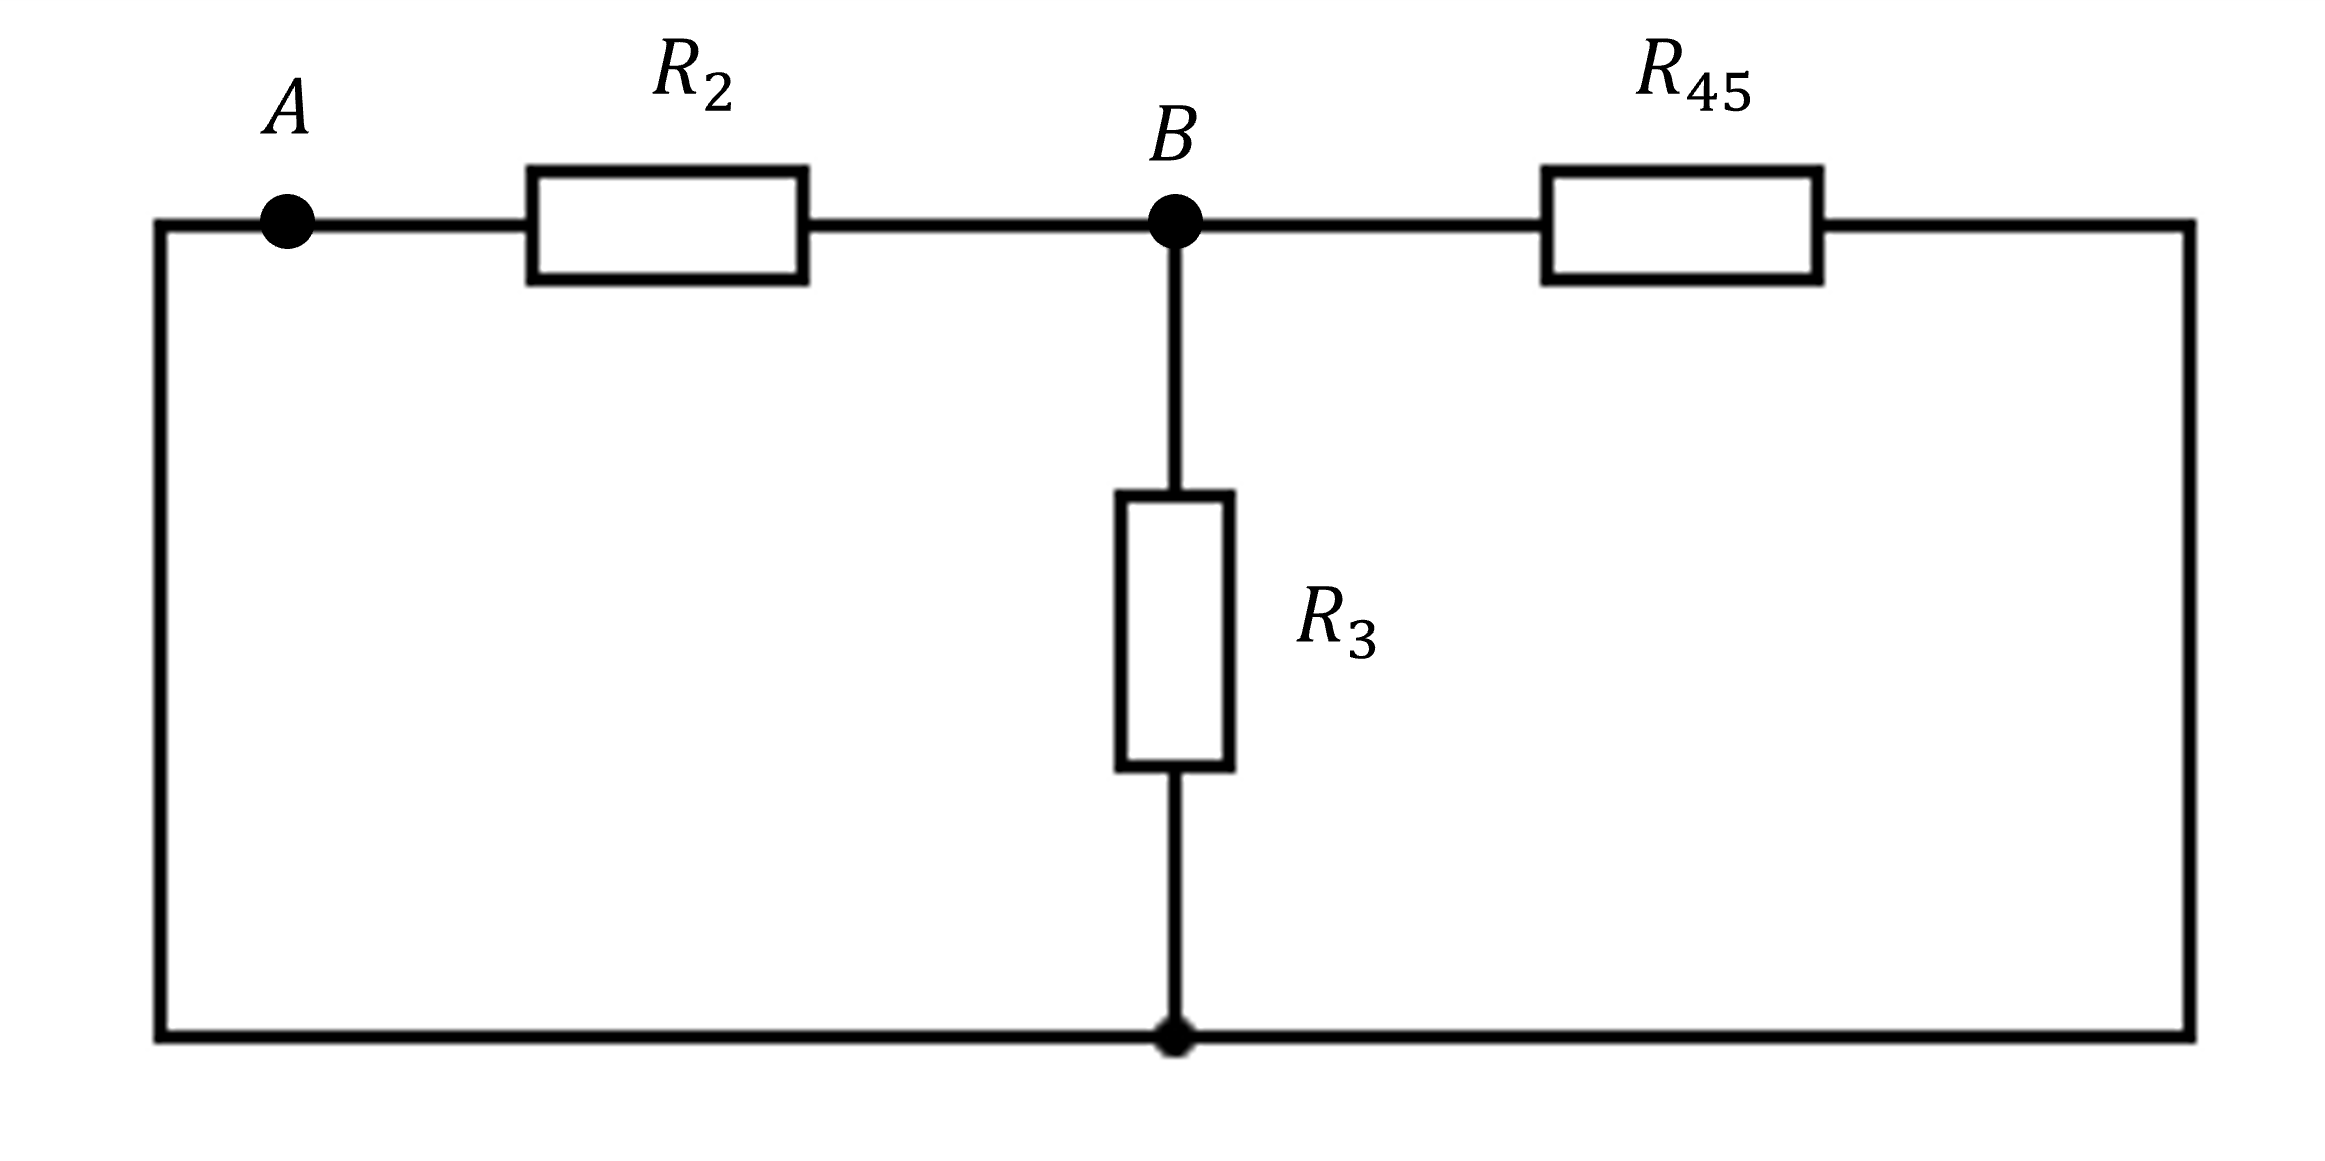
\includegraphics[scale=0.5,keepaspectratio]{fig/pr2_1.png} \
\end{center}

\begin{gather*}
    R_{45} = R_4 + R_5 = 200 + 550 = 750 \Omega \\
\end{gather*}

%%% Krok 2 - Výpočet Ri
\begin{center}
    \textbf{Krok 2} - Vypočítame vnútorný odpor $R_{i}$  - odpor medzi bodmi A a B
    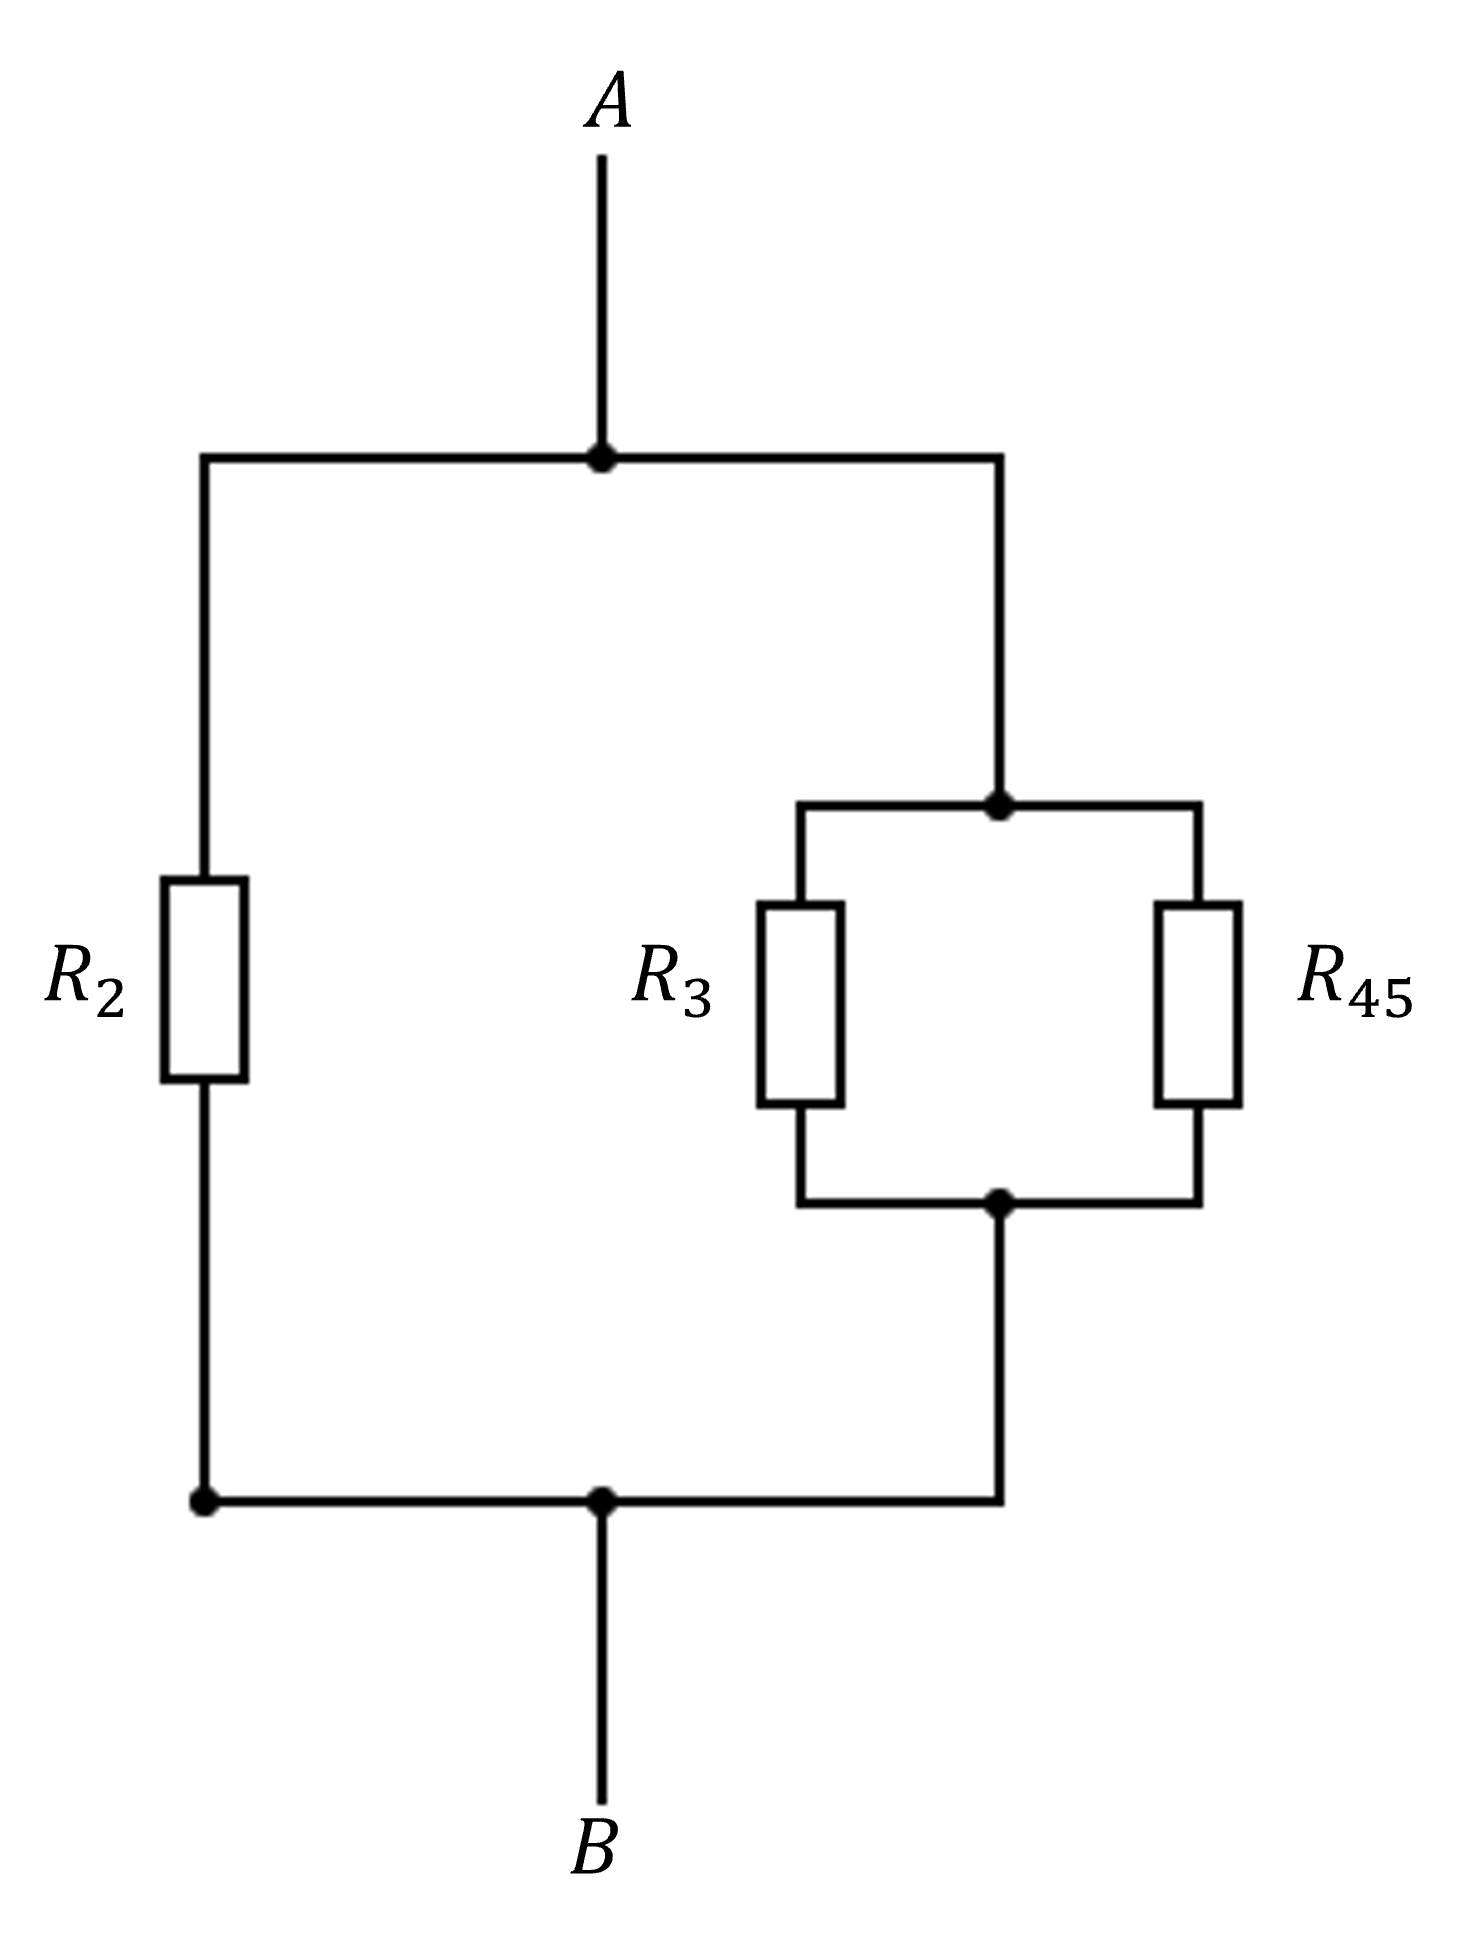
\includegraphics[scale=0.5,keepaspectratio]{fig/pr2_2.png} \
\end{center}

\begin{gather*}
    R_{453} = \frac {R_{3} \times R_{45}} {R_{3} + R_{45}} =  \frac {660 \times 750} {660 + 750} = 351,0638 \Omega \\\\
   R_{i} = \frac {R_{2} \times R_{453}} {R_{2} + R_{453}} = \frac {200 \times 351,0638} {200 + 351,0638} = 127,4131 \Omega \\\\
\end{gather*}

%%% Krok 2 - Vypočet Ui
\begin{center}
    \textbf{Krok 2} - Vypočítame $U_i$ pomocou smyčkového prúdu $I_A$
\end{center}

\begin{gather*}
    \begin{pmatrix}
    R_2 + R_3 & -R_3 \\
    -R_3 & R_3 + R_{45}
    \end{pmatrix}
    \times
    \begin{pmatrix}
    I_A \\
    I_B
    \end{pmatrix}
    =
    \begin{pmatrix}
    0 \\
    U
    \end{pmatrix}
\end{gather*}
\\

Vypočítame determinanty matice

\begin{gather*}
    M =
    \begin{vmatrix}
    860 & -660 \\
    -660 & 1410
    \end{vmatrix}
    =
    777000
    \\\\
    M_{I_A} =
    \begin{vmatrix}
    150 & -660 \\
    0 & 1410
    \end{vmatrix}
    =
    211500
\end{gather*}
\\

Použijeme Cramerovo pravidlo a determinanty matíc pre výpočet $I_A$:

\begin{gather*}
    I_A = \frac{M_{I_A}}{M} = \frac{211500}{777000} = 0.2722 A
    \\\\
    U_i \equiv U_{R_2} = I_A \times R_2 = 0.2722 \times 200 = 54,44 V
\end{gather*}

%%% Krok 3 - Vypočet U1 I1
\begin{center}
    \textbf{Krok 3} - Pomocou ekvivalentného obvodu dopočítame $U_1$ a $I_1$
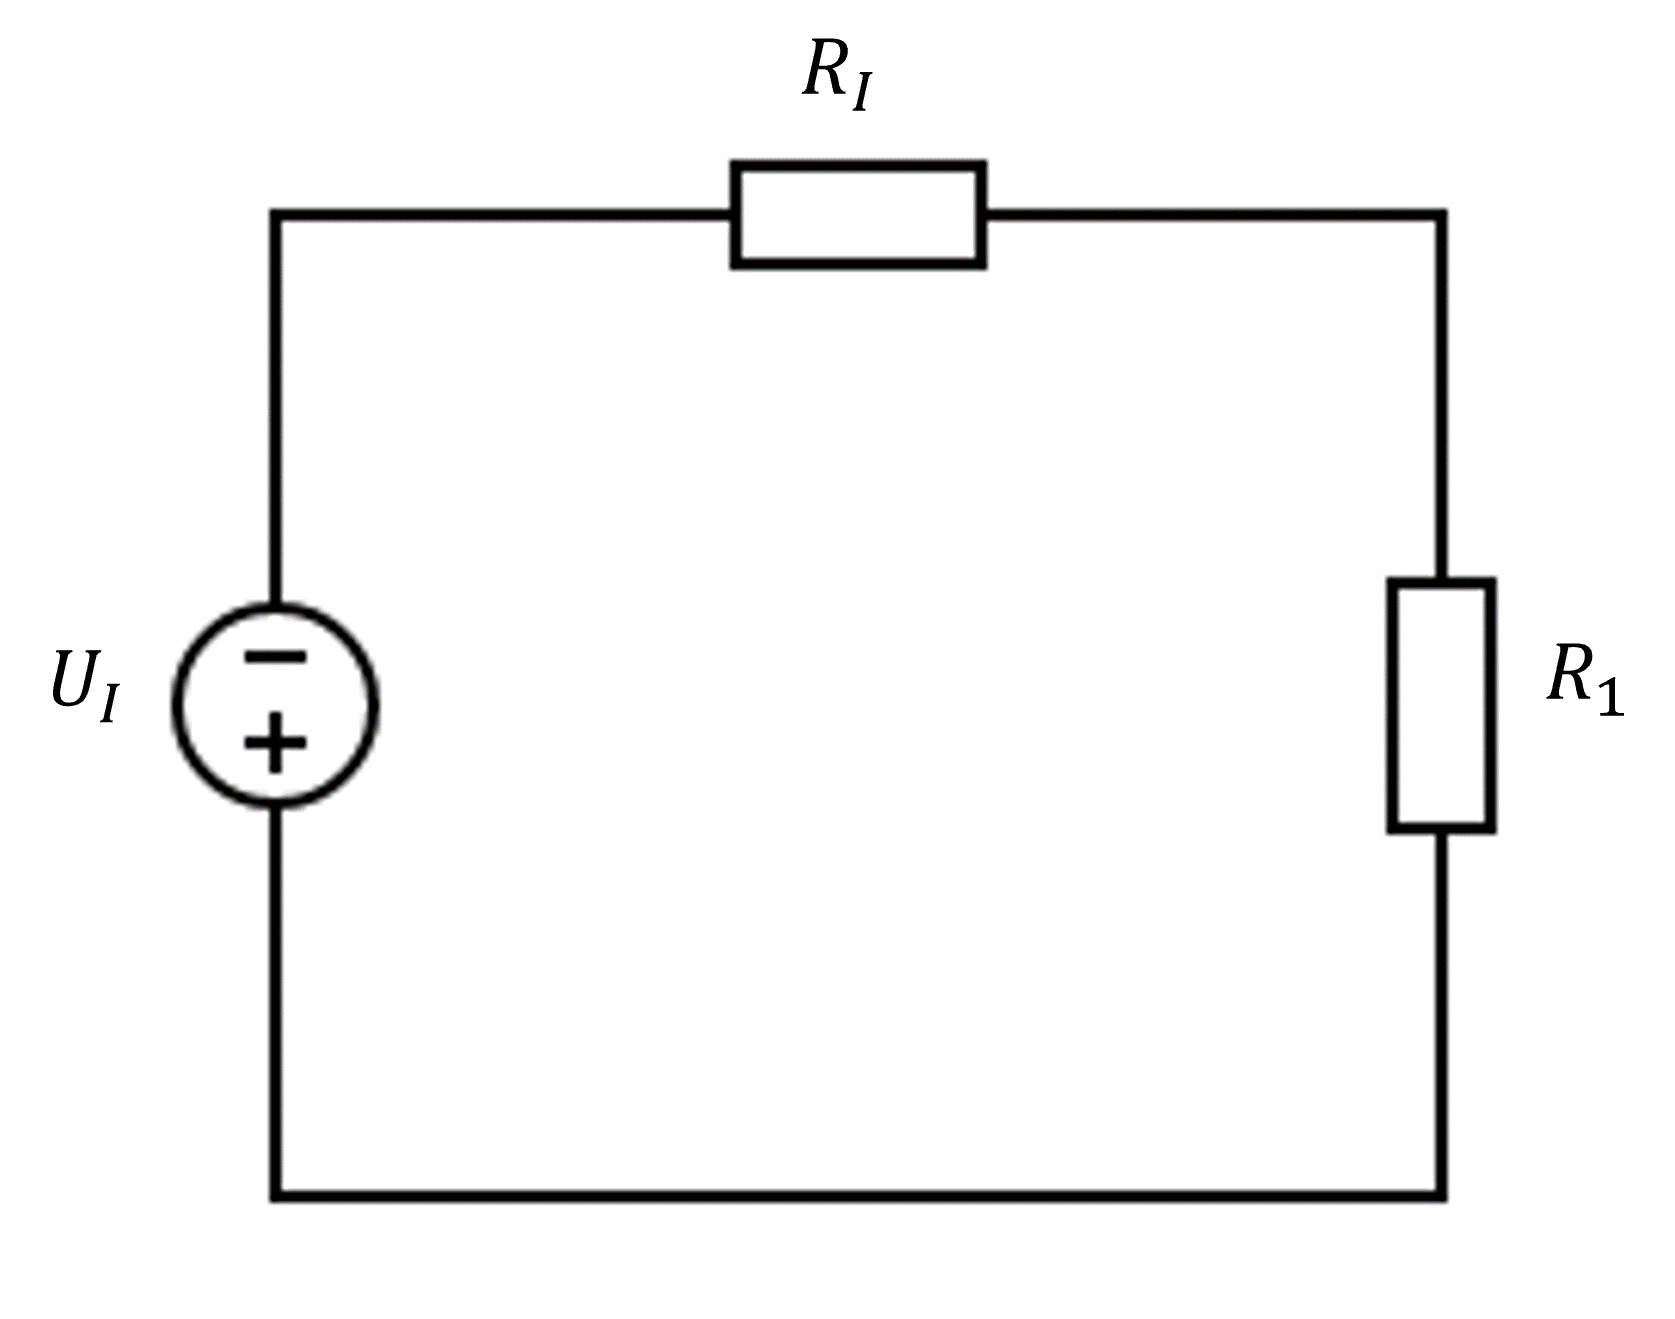
\includegraphics[scale=0.5,keepaspectratio]{fig/pr2_3.png} \
\end{center}

\begin{gather*}
    I_{R_{1}} = \frac {U_{i}} {R_{1} + R_{i}} = \frac {54,44} { 200 + 127,4131} = 166,2731 mA \\\\
    U_{R_{1}} = R_1 \times  I_{R_{1}} = 200 \times 0,166273 = 33,2546 V \\
\end{gather*}

